\documentclass[tikz,border=2pt]{standalone}
\usepackage{amsmath}
\usetikzlibrary{arrows.meta}
\begin{document}
% Inventory position under a (T,s,S) policy with T = 3, s = 1, S = 5 and demands 1,1,1,3,2,0,1,2:
% orders at the ends of periods 3 (time trigger), 5 (position 0 <= s) and 8 (time trigger).
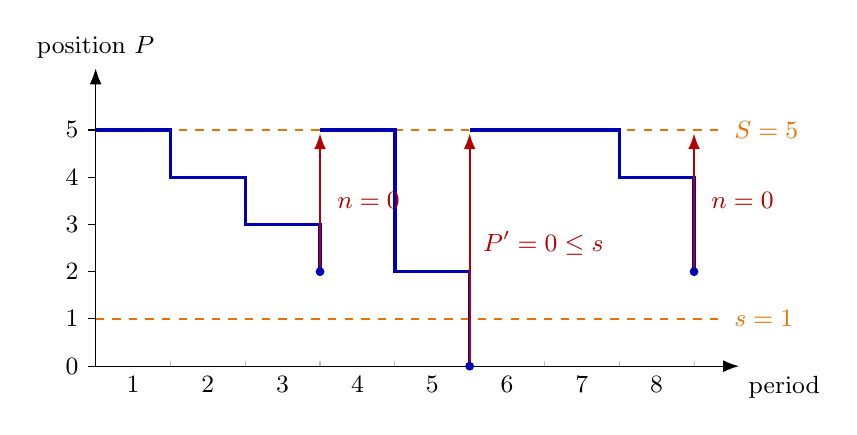
\begin{tikzpicture}[font=\small, >={Latex[length=2mm]}, x=0.95cm, y=0.6cm]
  % axes
  \draw[->] (0,0) -- (8.6,0) node[anchor=north west] {period};
  \draw[->] (0,0) -- (0,6.3) node[anchor=south] {position $P$};
  \foreach \k in {1,...,8} {\draw (\k-0.5,0) node[below] {$\k$};}
  \foreach \y in {0,1,2,3,4,5} {\draw (0,\y) -- (-0.1,\y) node[left] {$\y$};}
  \foreach \k in {1,...,8} {\draw[gray!50] (\k,0) -- (\k,0.12);}
  % policy levels
  \draw[orange!90!black, thick, dashed] (0,5) -- (8.4,5) node[right] {$S=5$};
  \draw[orange!90!black, thick, dashed] (0,1) -- (8.4,1) node[right] {$s=1$};
  % position path: start-of-period level, drop by demand at period end
  \draw[blue!70!black, very thick] (0,5) -- (1,5) -- (1,4) -- (2,4) -- (2,3) -- (3,3) -- (3,2);
  \draw[blue!70!black, very thick] (3,5) -- (4,5) -- (4,2) -- (5,2) -- (5,0);
  \draw[blue!70!black, very thick] (5,5) -- (6,5) -- (7,5) -- (7,4) -- (8,4) -- (8,2);
  % orders up to S
  \draw[->, red!70!black, thick] (3,2) -- (3,4.93);
  \draw[->, red!70!black, thick] (5,0) -- (5,4.93);
  \draw[->, red!70!black, thick] (8,2) -- (8,4.93);
  \fill[blue!70!black] (3,2) circle (1.6pt) (5,0) circle (1.6pt) (8,2) circle (1.6pt);
  % trigger labels
  \node[red!70!black, anchor=west] at (3.1,3.5) {$n=0$};
  \node[red!70!black, anchor=west] at (5.05,2.6) {$P'=0\leq s$};
  \node[red!70!black, anchor=west] at (8.1,3.5) {$n=0$};
\end{tikzpicture}
\end{document}
